%\noindent
\justifying
\setlength{\parskip}{1em}

This chapter discusses the implementation of the \ac{CycleGAN} and classifiers. In this thesis, classifiers are used to determine the domain gap between the distributions and to evaluate the quality of images generated by the \ac{CycleGAN}. The architecture of \ac{CycleGAN} and classifiers discussed in section \ref{NetworkArchitecture} and in section \ref{DatasetPreparation} dataset preparation is described. The training details of \ac{CycleGAN} and classifiers described in section \ref{TrainingDetails}. How the classifiers are used to analyze the domain gap between distributions will be discussed in chapter Evaluation \ref{evaluation}. The experiments are visualized using Tensorboard\footnotemark. TensorBoard is a tool that provides the visualization needed for machine learning research and experiments. The neural networks implemented in this thesis using Python, Keras APIs and TensorFlow library \cite{tensorflow2015-whitepaper}. The reference code for the \ac{CycleGAN} is available \href{https://keras.io/examples/generative/cyclegan/}{here}. All of the neural networks are trained upon GPUs (Graphics Processing Units) like Nvidia Tesla T4 and Tesla V100-SXM2. 

\footnotetext{\url{https://www.tensorflow.org/tensorboard} last access: \dcdate}


\section{Dataset Preparation}\label{DatasetPreparation}

\begin{figure}[H]
        \begin{center}
    	  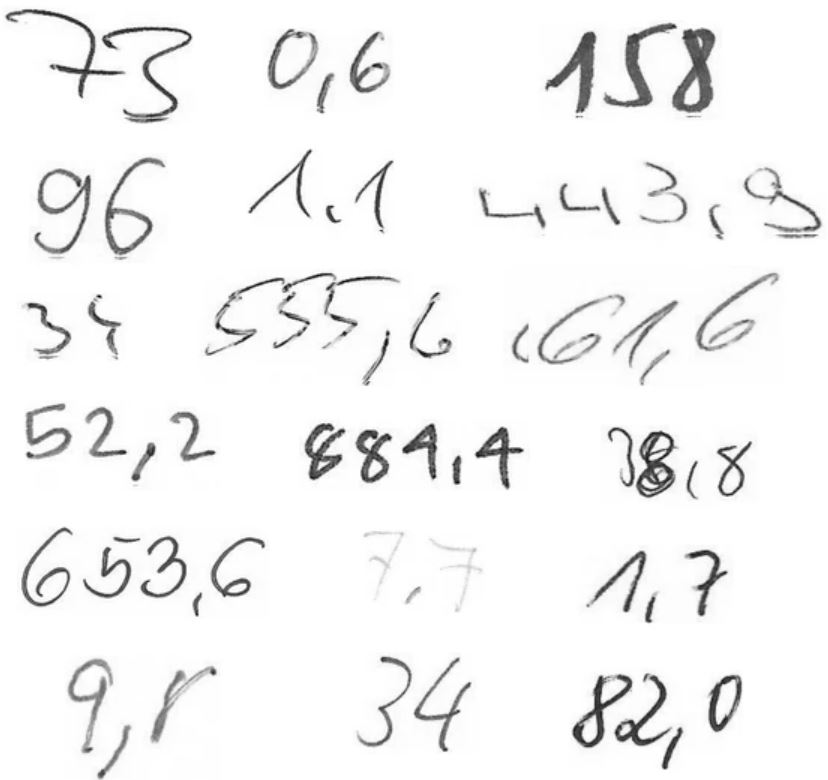
\includegraphics[scale=0.45]{images/Implementation/keinwifi.JPG}
	  \caption[Examples of handwritting crops from the handwritting number dataset.]{Examples of handwritting crops from the handwritting number dataset (figure reproduced from elevait GmbH \& Co. KG with permission).}
	  \label{fig:keinwifi}
	  \end{center}
\end{figure}


The dataset preparation is one of the vital step before training any neural network. Bad quality data leads to a poor generalization of neural networks \cite{10.5555/3153997}. Ten types of documents that were considered to work with this image-to-image translation application. The \ac{CycleGAN} is trained using a stash of synthetic document images and real document images stored in a memory. In the source domain, there are 100,000 synthetic document images and an equal amount of real document images are in the target domain. The synthetic document images are generated using templates (figure \ref{fig:template}) and handwritten crops (figure \ref{fig:keinwifi}). The process of inserting handwritten crops on empty templates can be visualized in figure \ref{fig:InsertHandwrittenCrops}. Each template is filled with the help of provided bounding box annotations \cite{lin2015microsoft}. For each class of template 10,000, synthetic document images are created. The dataset of 100,000 synthetic document images is formed. These synthetic document images are used while training \ac{CycleGAN}, just they are stashed at the single location collectively. The created 100,000 synthetic document images were also faxified and a faxified dataset of 100,000 images is created. It has 10 classes and each class has 10,000 images, similar to the synthetic document images dataset. 

The faxification process uses several image transformations to make a clean gray-scale image look like it was sent via fax. A sample faxified image can be seen in figure \ref{fig:FaxifiedImage}. The faxification process is described briefly in section \ref{trainingfaxifiedclassifier}. Also, the faxification process can be visualized in figure \ref{fig:FaxificationProcess}. In the table \ref{table:datasets} the number of samples in each dataset is mentioned. For testing, around 1162 annotated real document images are used. This testing dataset is used to evaluate the performance of the classifiers trained upon different data distributions like synthetic document images, faxified document images and \ac{CycleGAN} generated document images. Basically, testing dataset is significant to understand the domain gap between real data distribution and remaining data distributions. In the table \ref{table:testdataset} the number of samples in each class in the test dataset is mentioned. The testing dataset is unbalanced. The datasets used in this thesis can not be cited or published because they are not open for public use.

\begin{figure}[H]
        \begin{center}
	    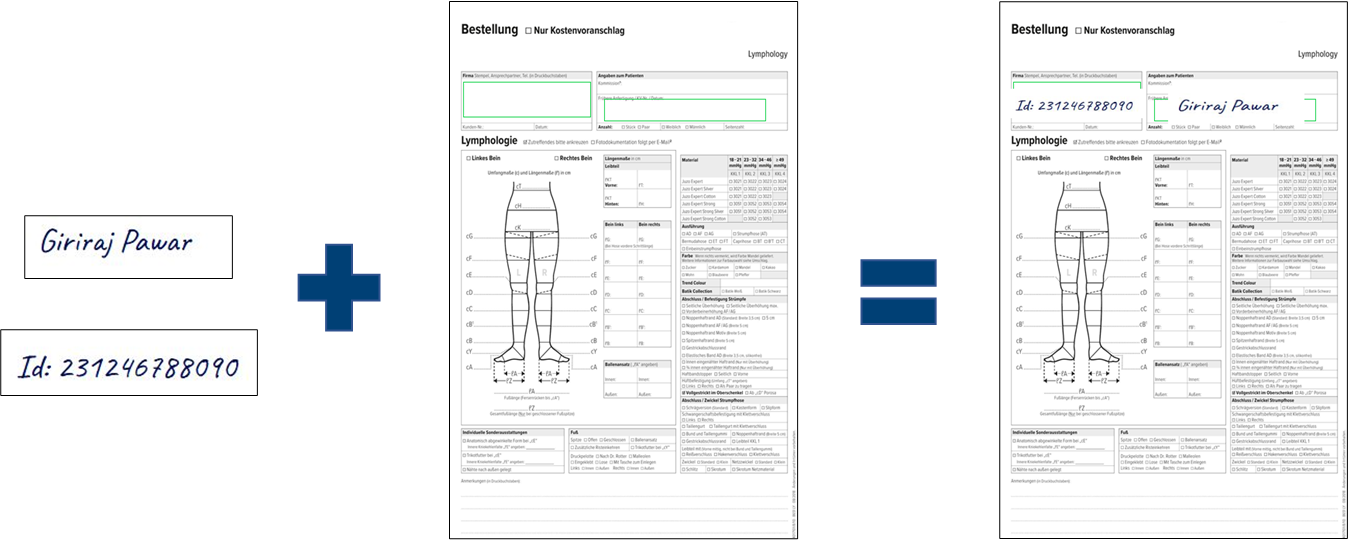
\includegraphics[scale=0.40]{images/Implementation/InsertHandwrittenCrops.png}
	    \caption[Inserting handwritten crops on empty form templates.]{Inserting handwritten crops on empty form templates (figure reproduced from elevait GmbH \& Co. KG with permission).}
	    \label{fig:InsertHandwrittenCrops}
	    \end{center}
\end{figure}





\begin{center}
    \begin{table}[H]
    \begin{center}
    \begin{tabular}{||c c||} 
    \hline
    \textbf{Datasets} & \textbf{Size (Number of Images)}\\ [0.5ex] 
    \hline\hline
    Synthetic Document Images & 100,000 \\ 
    \hline
    Real Document Images & 100,000 \\
    \hline
    Faxified Document Images & 100,000 \\
    \hline
    Annotated Real Document Images (Used for testing) & 1162 \\
    \hline
    \end{tabular}
    \end{center}
    \caption{Size of datasets used for training \ac{CycleGAN} and classifiers.}
    \label{table:datasets}
    \end{table}
\end{center}



\begin{center}
    \begin{table}[H]
    \begin{center}
    \begin{tabular}{||c c||} 
    \hline
    \textbf{Classes} & \textbf{Size (Number of Images)}\\ [0.5ex] 
    \hline\hline
    DE\_LY\_Arm\_2020-01 & 44 \\ 
    \hline
    DE\_LY\_Bein\_2018-08 & 47 \\
    \hline
    DE\_LY\_Bein\_2019-01 & 50 \\
    \hline
    DE\_LY\_Bein\_2019-07&  60\\
    \hline
    DE\_LY\_Bein\_2020-01&  624\\
    \hline
    DE\_LY\_Bein\_2020-03&  128\\
    \hline
    DE\_LY\_Hand\_2020-01&  16\\
    \hline
    DE\_PH\_Bein\_2018-09&  22\\
    \hline
    DE\_PH\_Bein\_2019-02&  28\\
    \hline    
    DE\_PH\_Bein\_2020-01&  143\\
    \hline    
    \end{tabular}
    \end{center}
    \caption[Number of images in each class of annotated real document images dataset.]{Number of images in each class of annotated real document images dataset (testing dataset).}
    \label{table:testdataset}
    \end{table}
\end{center}


The templates are unfilled form images. As described before, in this thesis, ten classes of templates are chosen for creating document images datasets like synthetic and faxified document images datasets. The 8 out of 10 templates are a type of ``Bein". Apart from minor differences, these templates are very similar to each other. Examples of ``Bein" templates are shown in figure \ref{fig:TemplatesWithMinorDifference}. The other two classes of templates are of type ``Hand'' and ``Arm''. In figure \ref{fig:TemplatesWithMajorDifference}, (a) is the template of ``Arm'', (b) is the template of ``Bein" and (c) is the template of ``Hand''. The list of classes or templates is listed in the table \ref{table:testdataset}.

\begin{figure}[H]
        \begin{center}
	    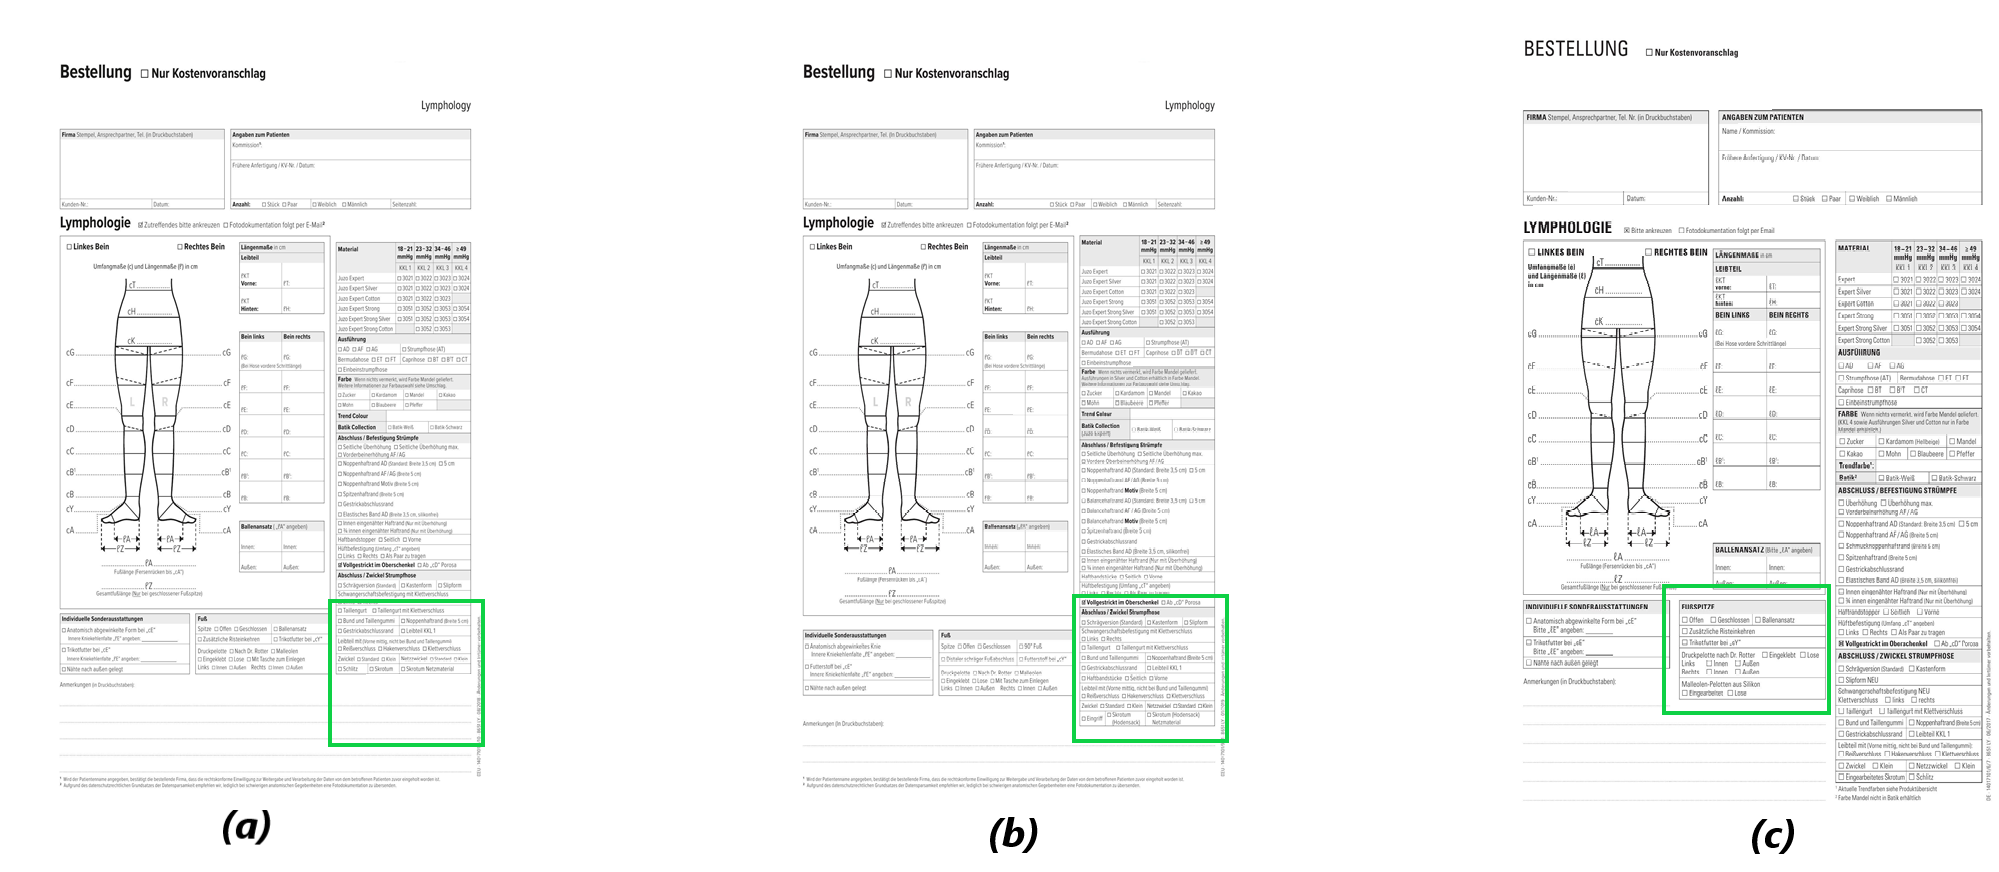
\includegraphics[scale=0.30]{images/Implementation/TemplatesWithMinorDifference.png}
	    \caption[Templates with minor differences.]{Templates with minor differences. All the templates (a), (b) and (c) are of type ``Bein'' (figure reproduced from elevait GmbH \& Co. KG with permission).}
	    \label{fig:TemplatesWithMinorDifference}
	    \end{center}
\end{figure}



\begin{figure}[H]
        \begin{center}
	    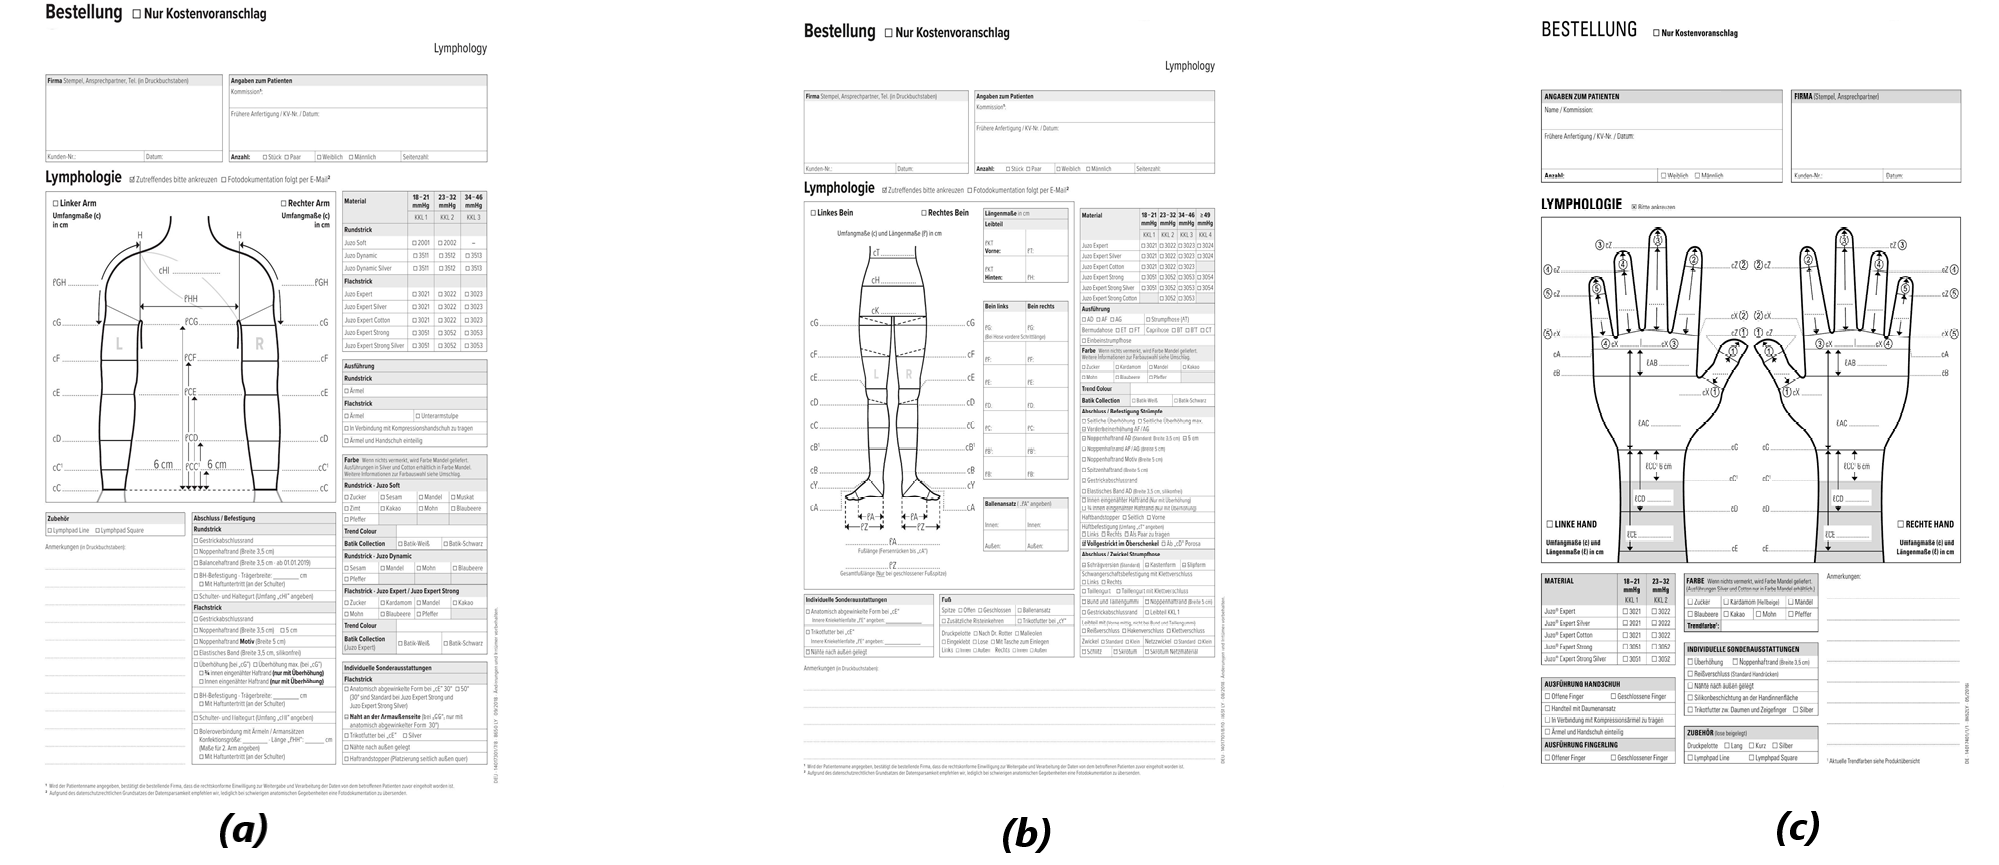
\includegraphics[scale=0.30]{images/Implementation/TemplatesWithMajorDifference.png}
	    \caption[Templates with major differences.]{Templates with major differences. (a) Template is of type ``Arm'', (b) Template is of type ``Bein'' and (c) Template is of type ``Hand'' (figure reproduced from elevait GmbH \& Co. KG with permission).}
	    \label{fig:TemplatesWithMajorDifference}
	    \end{center}
\end{figure}





\newpage

\section{Network Architecture}\label{NetworkArchitecture}

\subsection{\ac{CycleGAN}}

Johnson et al.\ \cite{johnson2016perceptual} proposed the architecture of \ac{CycleGAN}. In which the generator has three sequences of blocks one is downsampling, transformation and upsampling. The sequence of 2 downsampling convolutional blocks encode the $256 \times 256 \times 1$ grayscale input image, 9 \ac{ResNet} convolutional blocks to transform the image and 2 upsampling convolutional blocks to generate the output image of the same dimension as the input image. The reason behind using residual blocks is, they resolve the vanishing gradient problem in deep neural networks \cite{he2015deep}. The discriminator classifier network is designed using PatchGAN architecture \cite{isola2018imagetoimage} \cite{li2016precomputed}. The PatchGAN discriminator is simply a \ac{CNN}. The major difference between the PatchGAN discriminator and general \ac{GAN} discriminator is, \ac{GAN} discriminator maps input image to the scalar output, which represents image being real to fake. But, the PatchGAN discriminator maps the input image to $N \times N$ array of outputs, where each element in an output array represent a patch in an input image being real or fake. Basically, the PatchGAN discriminator penalizes structure at the scale of local image patches and attempts to classify as if each $M \times M$ patch in an image is real or fake.


Johnson et al.\ \cite{johnson2016perceptual} have provided naming conventions to define the architecture of generator and discriminator used in \ac{CycleGAN}. The complete generator network with 9 residual blocks can be described as: {\fontfamily{qcr}\selectfont c7s1-64, d128, d256, R256, R256, R256, R256, R256, R256, R256, R256, R256, u128, u64, c7s1-1}. {\fontfamily{qcr}\selectfont c7s1-k} denotes a $7 \times 7$ Convolution-InstanceNormlization-ReLU layer with $k$ filters and stride 1. The downsampling block {\fontfamily{qcr}\selectfont dk} is denoted by a $3 \times 3$ Convolution-InstanceNormlization-ReLU layer with $k$ filters and stride 2. To reduce artifacts reflection padding is used. {\fontfamily{qcr}\selectfont Rk} denotes a single residual block that has two $3 \times 3$ convolution layers with the same number of filters $k$ on both layers and stride 1. The upsampling block {\fontfamily{qcr}\selectfont uk} denoted a $3 \times 3$ TransposedConvolution-InstanceNormlization-ReLU layer with $k$ filters and stride 2. The last layer {\fontfamily{qcr}\selectfont c7s1-1} denotes a $7 \times 7$ Convolution layer with 1 filter and stride 1. Next, the final output is followed by a tanh activation function (figure \ref{fig:ActivationFunctions}). All of the layers in the generator can be seen in figure \ref{fig:GeneratorModelSummary}. The architecture of the generator is illustrated in table \ref{table:GeneratorArchitecture}. Also, in the figure \ref{fig:resnetBlock}, the architecture of \ac{ResNet} block in the generator network is illustrated. In which, at every \ac{ResNet} block, the output from the previous layer is passed through two convolution layers (each with {\fontfamily{qcr}\selectfont c3s1-256}). Further, it concatenated with the convolution layer's output and forwarded to the following layers.


\vspace*{1.0cm}
\begin{figure}[H]
        \begin{center}
	    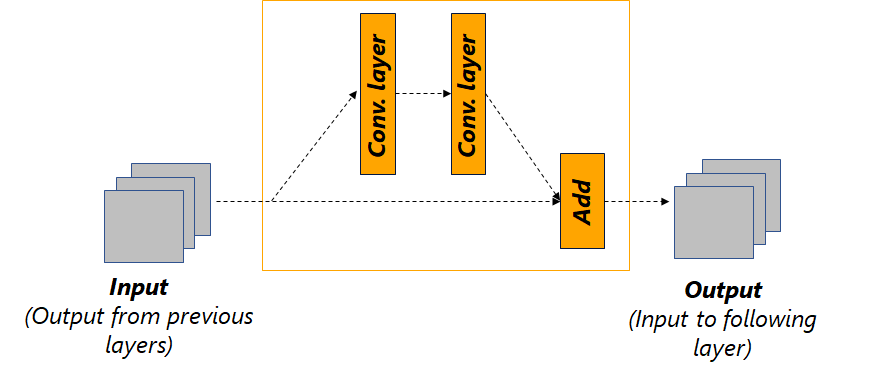
\includegraphics[scale=0.65]{images/Implementation/resnetBlocks.png}
	    \caption[An illustration of ResNet blocks in \ac{CycleGAN} generator architecture.]{An illustration of ResNet blocks in \ac{CycleGAN} generator architecture.}
	    \label{fig:resnetBlock}
	    \end{center}
\end{figure}


\begin{table}[H]
    \centering
    \begin{tabular}{P{0.35\linewidth} P{0.15\linewidth} P{0.15\linewidth} P{0.15\linewidth}} 
        \toprule
        \textbf{Operation Layer} & \textbf{Number of Filters/Units} & \textbf{Size of Each Filter} & \textbf{Stride Value}\\
        \toprule
        \toprule
        Input Image \\($256 \times 256 \times 1$) & - & - & - \\
        \midrule
        Convolution Layer\\Instance Normalization\\\ac{ReLU} & 64 & $7 \times 7$ & $1 \times 1$\\
        \midrule
        Convolution Layer\\Instance Normalization\\\ac{ReLU} & 128 & $3 \times 3$ & $2 \times 2$\\
        \midrule
        Convolution Layer\\Instance Normalization\\\ac{ReLU} & 256 & $3 \times 3$ & $2 \times 2$\\
        \midrule
        \textbf{9 Residual Blocks}\\
	  2 Convolution Layers\\ \textit{(each with)}\\Instance Normalization\\\ac{ReLU} & 256 & $3 \times 3$ & $1 \times 1$\\
        \midrule
        Transposed Convolution Layer\\Instance Normalization\\\ac{ReLU} & 128 & $3 \times 3$ & $2 \times 2$\\
        \midrule
        Transposed Convolution Layer\\Instance Normalization\\\ac{ReLU} & 64 & $3 \times 3$ & $2 \times 2$\\
        \midrule
         Convolution Layer\\tanh & 1 & $7 \times 7$ & $1 \times 1$\\
        \midrule
        \midrule
        Output  \\($256 \times 256 \times 1$) & - & - & -\\
        \bottomrule
    \end{tabular}
    \caption[Generator architecture]{Generator architecture}
    \label{table:GeneratorArchitecture}
\end{table}



The discriminator uses $70 \times 70$ PatchGAN classfier architecture \cite{isola2018imagetoimage}. It is also called a Markovian discriminator \cite{li2016precomputed}. The L1 and L2 loss functions produce blurry results while solving image generation problems \cite{ledig2017photorealistic}. These losses fail to encourage high-frequency crispness \cite{ledig2017photorealistic}. To model high frequencies, more attention is given to the structure in local image patches \cite{isola2018imagetoimage}. Therefore Markovian discriminator is called the PatchGAN discriminator. The design of discriminator network is: {\fontfamily{qcr}\selectfont C64-C128-C256-C512-C512-C1}. {\fontfamily{qcr}\selectfont Ck} denotes a $4 \times 4$ Convolution-InstanceNormalization-LeakyReLU layer with $k$ filters and stride 2. Leaky ReLUs with a slope of 0.2 are used. Instance Normalization is not used for the first {\fontfamily{qcr}\selectfont C64} layer. After the last layer {\fontfamily{qcr}\selectfont C512}, the convolution operation is applied with filter 1 to produce an output of depth 1 using $4 \times 4$ kernel and stride 1.  All of the layers in the discriminator can be seen in figure \ref{fig:DiscriminatorModelSummary}. The architecture of the classifier is illustrated in table \ref{table:DiscriminatorArchitecture}.





\begin{table}[H]
    \centering

    \begin{tabular}{P{0.30\linewidth} P{0.20\linewidth} P{0.20\linewidth} P{0.20\linewidth}} 
        \toprule
        \textbf{Operation Layer} & \textbf{Number of Filters/Units}  & \textbf{Size of Each Filter} & \textbf{Stride Value}\\
        \toprule
        \toprule
        Input Image \\($256 \times 256 \times 1$) & - & - & -\\
        \midrule
        Convolution Layer\\LeakyReLU (0.2) & 64 & $4 \times 4$ & $2 \times 2$\\
        \midrule
        Convolution Layer\\Instance Normalization\\LeakyReLU (0.2) & 128 & $4 \times 4$ & $2 \times 2$\\
        \midrule
        Convolution Layer\\Instance Normalization\\LeakyReLU (0.2) & 256 & $4 \times 4$ & $2 \times 2$\\
        \midrule
        Convolution Layer\\Instance Normalization\\LeakyReLU (0.2) & 512 & $4 \times 4$ & $1 \times 1$\\
        \midrule
        Convolution Layer\\Instance Normalization\\LeakyReLU (0.2) & 512 & $4 \times 4$ & $1 \times 1$\\
        \midrule
        \midrule
        Output  \\($16 \times 16 \times 1$) & - & - & -\\
        \bottomrule
    \end{tabular}
    \caption[Discriminator architecture]{Discriminator architecture}
    \label{table:DiscriminatorArchitecture}
\end{table}

For more information on the architectures of generators and discriminators, Github \href{https://github.com/junyanz/CycleGAN}{repository}\footnote{\url{https://github.com/junyanz/CycleGAN} last access: \dcdate} can be referred to. 



\subsection{Classifier}
In this thesis, the classifiers are used to analyze the domain gap between real data distribution and other data distributions like synthetic data distribution, faxified data distribution and \ac{CycleGAN} generated data distribution. Three separate classifiers are trained upon synthetic data distribution faxified data distribution and \ac{CycleGAN} generated data distribution respectively. Their classification performance was evaluated on annotated real document images (testing dataset) using metrics like weighted average F1-score, macro average F1-score and accuracy to investigate the domain gap between real data distribution and mentioned three data distributions. Chapter Evaluation \ref{evaluation} discusses more about evaluation metrics. The classifier architecture is simple and easy to implement. The architecture of the classifier is illustrated in table \ref{table:ClassifierArchitecture}. Also, all the layers in the classifier can be seen in figure \ref{fig:ClassifierModelSummary}.

\begin{table}[H]
    \centering

    \begin{tabular}{P{0.30\linewidth} P{0.20\linewidth} P{0.20\linewidth} P{0.20\linewidth}} 
        \toprule
        \textbf{Operation Layer} &  \textbf{Number of Filters/Units}  & \textbf{Size of Each Filter} & \textbf{Stride Value}\\
        \toprule
        \toprule
        Input Image \\($256 \times 256 \times 1$) & - & - \\
        \midrule
        Convolution Layer\\\ac{ReLU} & 32 & $3 \times 3$ & $1 \times 1$\\
        \midrule
        Convolution Layer\\\ac{ReLU} & 64 & $3 \times 3$ & $1 \times 1$\\
        \midrule
	  Max Pooling Layer & - & $2 \times 2$ & $2 \times 2$\\
	  \midrule
	  Dropout Layer (0.25) & - & - & -\\
	  \midrule
	  Flatten Layer & - & - & -\\
	  \midrule
	  Dense Layer\\\ac{ReLU} & 128 & - & -\\
	  \midrule
	  Dropout Layer (0.5) & - & - & -\\
	  \midrule
	  Dense Layer\\Softmax & 10 & - & -\\
        \midrule
        \midrule
	  Output \\($1 \times 10$) & - & - & -\\
      \bottomrule
    \end{tabular}
    \caption[Classifier architecture]{Classifier architecture}
    \label{table:ClassifierArchitecture}
\end{table}



\section{Training Details}\label{TrainingDetails}



%Now to stabilize the\ac{CycleGAN} model training procedure, which means training both generators $G$ and $F$ with the help of discriminators $D_Y$ and $D_X$ by reduced oscillations. 

\subsection{CycleGAN}\label{TrainingDetailsCycleGAN}
Designing an efficient and fast input pipeline is challenging. The proposed image-to-image translation application and classifiers are trained using 100,000 images. Loading such a large dataset is a tedious and time-consuming job but TensorFlow has provided wonderful \href{https://www.tensorflow.org/guide/data}{tf.data} APIs to load large datasets spontaneously. To learn more about how to load large datasets efficiently in TensorFlow refer to this \href{https://www.tensorflow.org/tutorials/load_data/images}{tutorial}. If the source domain is $X$ and the target domain is $Y$. The first generator $G$ is called the forward generator, which transforms images from $X \rightarrow Y$ and $D_Y$ acts as a discriminator for the generator $G$. The second generator $F$ is called the backward generator, which transforms images from $Y \rightarrow X$ and $D_X$ acts as a discriminator for the generator $F$. For the stable training of the \ac{CycleGAN} model, the general \ac{GAN} objective function \ref{ganObjectiveFunction} has been modified. In which, the negative log-likelihood objective is replaced by least-squares loss \cite{mao2017squares}. The \ac{GAN} loss function $\mathcal{L}_{ls}(G, D_Y, X, Y)$ of the forward generator $G$ minimizes $\mathbb{E}_{x \sim p_{data}(x)}\ (D_Y(G(x)) - 1)^2$ and discriminator $D_Y$ minimizes $\frac{1}{2}\ \mathbb{E}_{y \sim p_{data}(y)}\ (D_Y(y) - 1)^2 + \frac{1}{2}\ \mathbb{E}_{x \sim p_{data}(x)}\ (D_Y(G(x)))^2$. Similarly, the \ac{GAN} loss function $\mathcal{L}_{ls}(F, D_X, Y, X)$ of the backward generator $F$ minimizes $\mathbb{E}_{y \sim p_{data}(y)}\ (D_X(F(y)) - 1)^2$ and discriminator $D_X$ minimizes $\frac{1}{2}\ \mathbb{E}_{x \sim p_{data}(x)}\ (D_X(x) - 1)^2 + \frac{1}{2}\ \mathbb{E}_{y \sim p_{data}(y)}\ (D_X(F(y)))^2$.

The learning rate ($\eta$) is set to $0.0002$ while training \ac{CycleGAN}. The weights neural networks (generators and discriminators) in the \ac{CycleGAN} model are initialized by a Gaussian distribution with standard deviation ($\sigma$) 0.02 and mean ($\mu$) 0. In the final objective function \ref{FullObjective}, $\lambda_{cyc}$ is set to $10$ and $\lambda_{identity}$ is set to $0.5$, which means importance of cycle-consistency loss is higher than identity mapping loss in the final objective function. The weights of the neural networks of \ac{CycleGAN} model are optimized by ADAM solver, which is a method for stochastic optimization \cite{kingma2017adam}. Also, while constructing generators and discriminators the instance normalization layers \cite{ulyanov2017instance} are used and gamma weight is initialized by Gaussian distribution with mean ($\mu$) 0 and standard deviation ($\sigma$) 0.02.


\begin{figure}[H]
        \begin{center}
	    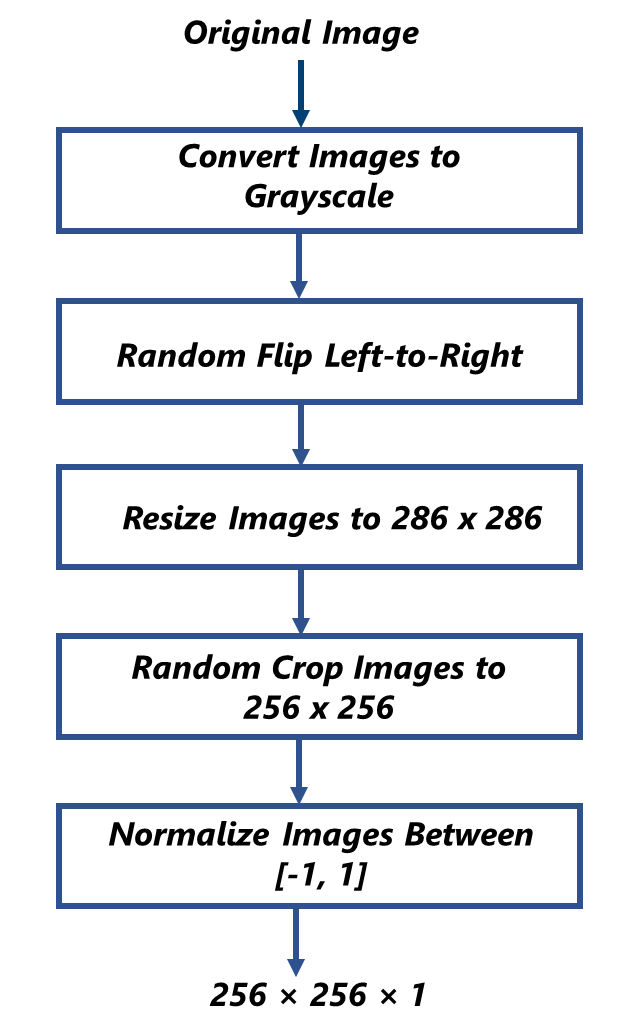
\includegraphics[scale=0.35]{images/Implementation/Preprocessing.png}
	    \caption[Steps involved in preprocessing of training images of \ac{CycleGAN}.]{Steps involved in preprocessing of training images of \ac{CycleGAN}.}
	    \label{fig:Preprocessing}
	    \end{center}
\end{figure}


The \ac{CycleGAN} model is trained with batch size 1 for 20 epochs. The complete \ac{CycleGAN} model consists of forward generator $G$, backward generator $F$, discriminator $D_Y$ and discriminator $D_X$. The training checkpoints\footnote{\url{https://www.tensorflow.org/guide/checkpoint} last access: \dcdate} are saved at the end of every epoch. The stack of 100,000 synthetic document images (Domain $X$) and 100,0000 real document images (Domain $Y$) are used to train the \ac{CycleGAN} model. The training images are preprocessed and the preprocessing process is illustrated in figure \ref{fig:Preprocessing}. Initially, the training images are converted into grayscale. Next, random mirroring is applied, in which the image is randomly flipped horizontally from left to right. Further, random mirroring is applied, in which the image is resized to $286 \times 286$ and then randomly cropped to $256 \times 256$. Random jittering and mirroring are image augmentation techniques that avoid overfitting \cite{zhu2020unpaired}. Finally, the images are normalized to a value between -1 and 1.

\subsection{Classifier}

Three separate classifiers are trained, first on synthetic document images, second on faxified document images and third on \ac{CycleGAN} generated document images. The synthetic and faxified document images are preprocessed. The preprocessing process of these images is illustrated in figure \ref{fig:PreprocessingClassfier}. Initially, the training images are converted into grayscale. Next, resized to $256 \times 256$ and later normalized between $[-1, 1]$. The \ac{CycleGAN} generated document images are need not be preprocessed, as the images generated by the generator $G$ ($G : X \rightarrow Y$) are of $256 \times 256$ dimension and already normalized between $[-1, 1]$. Because at the final layer of the generator, the tanh activation function is used, this can be seen in the architecture of the generator in table \ref{table:GeneratorArchitecture}. All three classifiers are trained for 10 epochs with 100,000 images and evaluated using 1162 annotated real document images (testing dataset).

\begin{figure}[H]
        \begin{center}
	    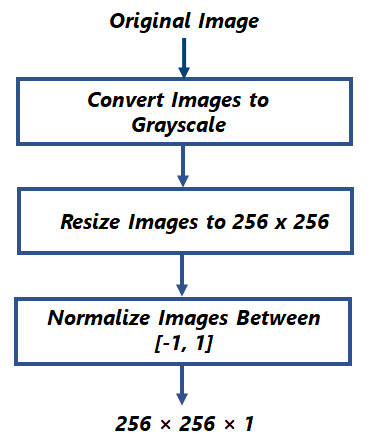
\includegraphics[scale=0.55]{images/Implementation/ClassifierPreprocessing.png}
	    \caption[Steps involved in preprocessing of training images (Only synthetic and faxified document images) of classifiers.]{Steps involved in preprocessing of training images (Only synthetic and faxified document images) of classifiers.}
	    \label{fig:PreprocessingClassfier}
	    \end{center}
\end{figure}

















































































%%%%%%%%%%%%%%%%%%%%%%%%%%%%%%%%%%%%%%%%%%%%%%%%%%%%%%%%%%%%%%%%%%%%%%%%%%%%%%%%%%%%%%%%%%%%%%%%%%%%%%%

%In the faxification process, several image transformations are applied to the images randomly means the output images produced during this process are random. Transformations like rotation, brightness difference, dithering  \cite{8580565} are visible in the above image after the faxification process. The dithering is the process of applying noise intentionally in the images.


\begin{comment}
\begin{figure}[H]
        \begin{center}
    	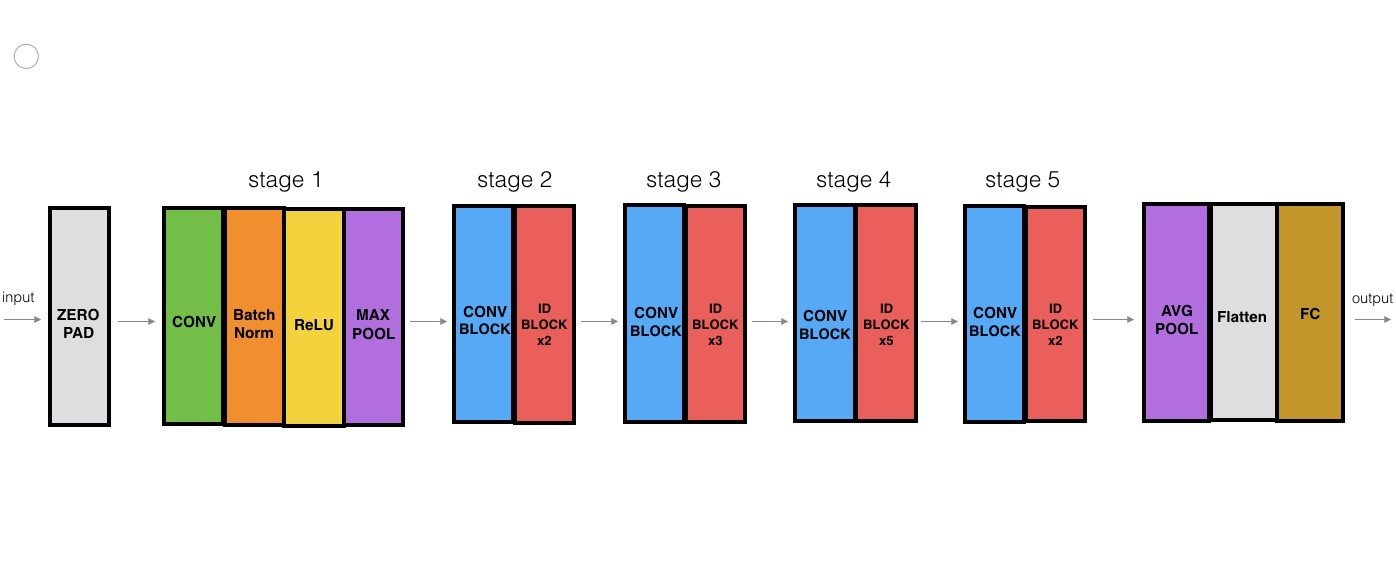
\includegraphics[scale=0.43]{images/ResNet50_1.jpg}
	    \caption[ResNet-50 Classifier Architecture.]{ResNet-50 Classifier Architecture.\footnotemark}
	    \label{fig:ResNet50}
	    \end{center}
\end{figure}
\footnotetext{\url{https://github.com/priya-dwivedi/Deep-Learning/blob/master/resnet_keras/Residual_Networks_yourself.ipynb} last access: 04.05.2021}

\begin{figure}[H]
        \begin{center}
	    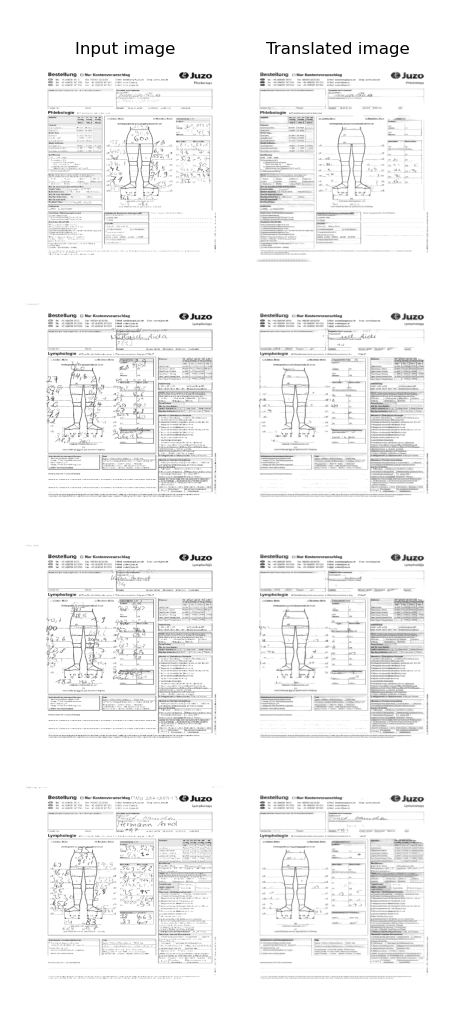
\includegraphics[scale=0.60]{images/CycleGAN_Generated_Images_3_5.png}
	    \caption{\ac{CycleGAN} transalated images.}
	    \label{fig:GeneratedImages}
	    \end{center}
\end{figure}


\end{comment}

\begin{comment}
\begin{figure}[H]
      \centering
      \hspace*{-0.75cm}
      \begin{tikzpicture}
        \node[rotate=0,minimum width=4.5cm] (input) at (0,11.25) {\small{Original Image}};
        \node[conv,rotate=0,minimum width=4.5cm] (Grayscale) at (0,10) {\small{Convert Images to Grayscale}};
        \node[conv,rotate=0,minimum width=4.5cm] (Randomflip) at (0,8.75) {\small{Random Flip Left-to-Right}};
        \node[pool,rotate=0,minimum width=4.5cm] (Resize) at (0,7.5) {\small{Resize Images to 286 x 286}};
        \node[dp,rotate=0,minimum width=4.5cm] (Randomcrop) at (0,6.25) {\small{Random Crop Images to 256 x 256}};
        \node[flatten,rotate=0,minimum width=4.5cm] (normalize) at (0,5.0) {\small{Normalize Images Between [-1, 1]}};
        \node[rotate=0,minimum width=4.5cm] (output) at (0,3.75) {\small$256 \times 256 \times 1$};

        \draw[->] (input) -- (Grayscale);
        \draw[->] (Grayscale) -- (Randomflip);
        \draw[->] (Resize) -- (Randomcrop);
        \draw[->] (Randomcrop) -- (normalize);
        \draw[->] (normalize) -- (output);
        
      \end{tikzpicture}
      \vskip 6px
      \caption{Pre-processing Process of Images.}
      \label{fig:Pre-processingSteps}
\end{figure}

\end{comment}
%While conducting the experiments, ResNet-50  \cite{he2015deep} architecture also has been considered. The architecture of ResNet-50 classifier can be viewed in figure \ref{fig:ResNet50}.


%The proposed image-to-image translation application is implemented using \ac{CycleGAN}. The quality of images generated by the \ac{CycleGAN} is assessed by a classifier that is trained on the same generated images and tested on real images. The classification performance of the classifier on real images is the metric to evaluate the quality of generated images. The evaluation of images generated by \ac{CycleGAN} is described thoroughly in section \ref{evaluation}. In this thesis, numerous experiments were performed to understand the domain gap\footnotemark 
%\footnotetext{\url{https://machinelearning.apple.com/research/bridging-the-domain-gap-for-neural-models} last access: 27.05.2021} between real document images and different data distributions like synthetic document images, faxified document images and \ac{CycleGAN} generated document images. 

%The proposed image-to-image translation application is implemented using \ac{CycleGAN}. The quality of images generated by the \ac{CycleGAN} is assessed by a classifier that is trained on the same generated images and tested on real images. The classification performance of the classifier on real images is the metric to evaluate the quality of generated images. The evaluation of images generated by \ac{CycleGAN} is described thoroughly in section \ref{evaluation}. In this thesis, numerous experiments were performed to understand the domain gap\footnotemark 
%\footnotetext{\url{https://machinelearning.apple.com/research/bridging-the-domain-gap-for-neural-models} last access: 27.05.2021} between real document images and different data distributions like synthetic document images, faxified document images and \ac{CycleGAN} generated document images. The experiments are visualized using Tensorboard\footnotemark. TensorBoard is tool which provides the visualization needed for machine learning experimentation. The \ac{CycleGAN} and Classifier are implemented in Python and using the TensorFlow library \cite{tensorflow2015-whitepaper}. The code for the \ac{CycleGAN} is available \href{https://keras.io/examples/generative/cyclegan/}{here}. All of the neural networks are trained upon GPUs (Graphics Processing Units) like Nvidia Tesla T4 and Tesla V100-SXM2.

%\footnotetext{\url{https://www.tensorflow.org/tensorboard} last access: 04.05.2021}


\begin{comment}

The architecture of \ac{CycleGAN} is adapted from Johnson et al.\ ~ \cite{johnson2016perceptual}. The generator network is implemented using a sequence of downsampling convolutional blocks to encode the $256 \times 256 \times 1$ grayscale input image, 9 \ac{ResNet} convolutional blocks to transform the image and a number of upsampling convolutional blocks to generate the output image of the same dimension as the input image. The reason behind using residual blocks is it resolves the vanishing gradient problem in deep neural networks. The discriminator networks uses PatchGAN ~ \cite{isola2018imagetoimage}. In PatchGAN, after feeding one input image to the network, it gives you the probabilities of two things: either real or fake, but not in scalar output indeed, it used the $N \times N$ output vector. Here $N \times N$ can be different depending on the dimension of an input image. The naming convention used in the Johnson et al.\'s \cite{johnson2016perceptual} Github \href{https://github.com/jcjohnson/fast-neural-style}{repository}. The architecture of discriminator and generator can be preciously visualised in figures \ref{fig:discriminator} and \ref{fig:generator}. 

Let {\fontfamily{qcr}\selectfont c7s1-k} denote a $7 \times 7$ Convolution-InstanceNorm-ReLU layer with k filters and stride 1. {\fontfamily{qcr}\selectfont dk} denotes a $3 \times 3$ Convolution-InstanceNorm-ReLU layer with $k$ filters and stride 2. Reflection padding was used to reduce artifacts. {\fontfamily{qcr}\selectfont Rk} denotes a residual block that contains two $3 \times 3$ convolutional layers with the same number of filters on both layer. {\fontfamily{qcr}\selectfont uk} denotes a $3  \times 3$ fractional-strided-Convolution-InstanceNorm-ReLU layer with $k$ filters and stride $\frac{1}{2}$. The generator network with 9 residual blocks consists of: {\fontfamily{qcr}\selectfont c7s1-64, d128, d256, R256, R256, R256, R256, R256, R256, R256, R256, R256, u128, u64, c7s1-1}. followed by a Tanh function (figure \ref{fig:ActivationFunctions}). The discriminator uses $70 \times 70$ PatchGAN \cite{isola2018imagetoimage}, which is also called as Markovian discriminator \cite{isola2018imagetoimage}. Let {\fontfamily{qcr}\selectfont Ck} denote a $4 \times 4$ Convolution-InstanceNorm-LeakyReLU layer with $k$ filters and stride 2. After the last layer, a convolution is applied to produce a 1-dimensional output. We do not use InstanceNorm for the first C64 layer. We use leaky ReLUs with a slope of 0.2. The discriminator architecture is: {\fontfamily{qcr}\selectfont C64-C128-C256-C512}.


\end{comment}


\begin{comment}

\begin{center}
\begin{table}[H]
    \begin{center}
    \begin{tabular}{p{0.25\linewidth} p{0.25\linewidth} p{0.25\linewidth} p{0.25\linewidth}} 
        \toprule
        Operation Layer & Number of Filters & Size of Each Filter & Stride Value\\
        \midrule
        Input Image ($256 \times 256$) & - & - \\
        \midrule
        Convolution Layer & 32 & $3 \times 3$ & $1 \times 1$\\
        \bottomrule
    \end{tabular}
    \caption[]{}
    \label{table:ClassifierArchitecture}
    \end{center}
\end{table}
\end{center}



\begin{center}
\begin{table}[H]
    \begin{center}
    \begin{tabular}{p{0.15\linewidth} p{0.10\linewidth} p{0.10\linewidth} p{0.10\linewidth} p{0.10\linewidth}} 
        \toprule
         Operation Layer & Number of Filters & Size of Each Filter & F1-score & Support\\[0.0ex] 
        \midrule
      
        \bottomrule
    \end{tabular}
    \caption[]{}
    \label{table:discriminatorArchitecture}
    \end{center}
\end{table}
\end{center}



\begin{figure}[H]
      \centering
      \hspace*{-0.75cm}
      \begin{tikzpicture}
        \node[rotate=90,minimum width=4.5cm] (input) at (0,0) {\small$\ 256 \times 256 \times 1$};
        \node[conv,rotate=90,minimum width=4.5cm] (conv1) at (1.25,0) {\small$\text{Conv2D}_{32, \text{$3 \times 3$}}$\,+\,$\ReLU$};
        \node[conv,rotate=90,minimum width=4.5cm] (conv2) at (2.5,0) {\small$\text{Conv2D}_{64, \text{$3 \times 3$}}$\,+\,$\ReLU$};
        \node[pool,rotate=90,minimum width=4.5cm] (pool1) at (3.75,0) {\small$\text{Max Pooling}_{\text{$2 \times 2$}}$};
        \node[dp,rotate=90,minimum width=4.5cm] (dp) at (5.0,0) {\small$\text{Dropout}_{\text{$0.25$}}$};
        \node[flatten,rotate=90,minimum width=4.5cm] (flatten) at (6.25,0) {\small$\text{Flatten}$};
        \node[fc,rotate=90,minimum width=4.5cm] (fc) at (7.5,0) {\small$\text{FC Layer}_{128}$\,+\,$\ReLU$};
        \node[dp,rotate=90,minimum width=4.5cm] (dp1) at (8.75,0) {\small$\text{Dropout}_{\text{$0.25$}}$};
        \node[fc,rotate=90,minimum width=4.5cm] (fc1) at (10,0) {\small$\text{FC Layer}_{10}$\,+\,$\ReLU$};
        \node[rotate=90,minimum width=4.5cm] (output) at (11.25,0) {\small$1 \times 10$};

        
        \draw[->] (input) -- (conv1);
        \draw[->] (conv1) -- (conv2);
        \draw[->] (conv2) -- (pool1);
        \draw[->] (pool1) -- (dp);
        \draw[->] (dp) -- (flatten);
        \draw[->] (flatten) -- (fc);
        \draw[->] (fc) -- (dp1);
        \draw[->] (dp1) -- (fc1);
        \draw[->] (fc1) -- (output);
        
  
        
      \end{tikzpicture}
      \vskip 6px
      \caption[Classifier Architecture.]{Classifier Architecture.}
      \label{fig:ClassifierArchitecture}
\end{figure}


\begin{figure}[H]
      \centering
      \hspace*{-0.75cm}
      \begin{tikzpicture}
        \node[rotate=90,minimum width=5cm] (input) at (0,0) {\small$\ 256 \times 256 \times 1$};
        \node[conv,rotate=90,minimum width=5cm] (conv1) at (1.25,0) {\small$\text{Conv2D}_{64, \text{$4 \times 4$}}$ + $\LeakyReLU$};
        \node[conv,rotate=90,minimum width=5cm] (conv2) at (2.5,0)   {\small$\text{Conv2D}_{128, \text{$4 \times 4$}}$ + InstanceNorm + ${\LeakyReLU}_{0.2}$};
	 \node[conv,rotate=90,minimum width=5cm] (conv3) at (3.75,0)  {\small$\text{Conv2D}_{256, \text{$4 \times 4$}}$ + InstanceNorm + ${\LeakyReLU}_{0.2}$};
	 \node[conv,rotate=90,minimum width=5cm] (conv4) at (5.0,0)  {\small$\text{Conv2D}_{512, \text{$4 \times 4$}}$   + InstanceNorm + ${\LeakyReLU}_{0.2}$};
	 \node[conv,rotate=90,minimum width=5cm] (conv5) at (6.25,0)  {\small$\text{Conv2D}_{512, \text{$4 \times 4$}}$   + InstanceNorm + ${\LeakyReLU}_{0.2}$};
	 \node[conv,rotate=90,minimum width=5cm] (conv6) at (7.5,0)  {\small$\text{Conv2D}_{1, \text{$4 \times 4$}}$};
	 \node[rotate=90,minimum width=5cm] (output) at (8.75,0) {\small$16 \times 16 \times 1$};

        
        \draw[->] (input) -- (conv1);
        \draw[->] (conv1) -- (conv2);
        \draw[->] (conv2) -- (conv3);
        \draw[->] (conv3) -- (conv4);
        \draw[->] (conv4) -- (conv5);
        \draw[->] (conv5) -- (conv6);
        \draw[->] (conv6) -- (output);

        
  
        
      \end{tikzpicture}
      \vskip 6px
      \caption[Discriminator Architecture.]{Discriminator Architecture.}
      \label{fig:DiscriminatorArchitecture}
\end{figure}

\end{comment}
